\chapter{Attention Mechanism}

Before the transformer, the dominant architecture for sequence modeling was the
recurrent neural network (RNN). RNNs process tokens one at a time, maintaining a
hidden state that carries information forward. This sequential bottleneck has two
consequences: training cannot be parallelized across time steps, and the model
struggles to carry information across long distances because the hidden state is
repeatedly overwritten.

The attention mechanism solves both problems. Instead of compressing everything
into a fixed-size hidden state, attention allows every position in a sequence to
directly inspect every other position in a single step. No information needs to
be ``squeezed through a bottleneck''---it is retrieved on demand. This idea is
the core innovation behind transformers and, by extension, every modern large
language model.

This chapter builds the attention mechanism from the ground up. It starts with
simplified self-attention (no learnable parameters), adds the Q/K/V projections
and scaling to arrive at scaled dot-product attention, introduces causal masking
for autoregressive generation, and then combines everything into multi-head
attention---the form used in real transformers. Along the way, it discusses
attention as a soft dictionary lookup and addresses the $O(n^2)$ complexity that
motivates many modern optimizations.

\section{Simplified Self-Attention}

The simplest form of self-attention uses no learnable parameters at all: the
input embeddings directly produce attention weights. While this version is too
simple for a real model, it reveals the core idea clearly.

Consider a sequence of $n$ embedding vectors $X \in \mathbb{R}^{n \times d}$,
where each row is the $d$-dimensional embedding of one token. Self-attention
computes, for each position, a weighted sum of all positions in the sequence:

\[
  \text{scores} = X \cdot X^\top, \qquad
  \text{attn\_weights} = \text{softmax}(\text{scores}), \qquad
  \text{output} = \text{attn\_weights} \cdot X
\]

Intuitively, the score matrix $X X^\top$ measures how similar each pair of
positions is (via dot product). Softmax normalizes each row of scores into a
probability distribution. The output at position $i$ is then a convex combination
of all input embeddings, weighted by how relevant each position is to position $i$.

\begin{pseudocode}[Simplified Self-Attention (No Learnable Parameters)]
def simplified_self_attention(X: Tensor) -> Tensor:
    # X: [batch, seq_len, embed_dim]
    # Note: for clarity, the equations above omit the batch dimension.
    # The implementation includes it for consistency with later sections.
    scores = X @ X.transpose(-2, -1)  # [batch, seq_len, embed_dim] @ [batch, embed_dim, seq_len] -> [batch, seq_len, seq_len]
    attn_weights = softmax(scores, dim=-1)  # [batch, seq_len, seq_len]
    output = attn_weights @ X  # [batch, seq_len, seq_len] @ [batch, seq_len, embed_dim] -> [batch, seq_len, embed_dim]
    return output
\end{pseudocode}

\begin{keyconcept}
  Self-attention lets each position in a sequence attend to (i.e.,
  compute a weighted average of) all other positions. Without learnable
  parameters, it computes similarity purely from the embedding geometry.
  The similarity function is the dot product, which measures how aligned
  two vectors are. Because the weights are produced by softmax, each row
  sums to 1, making the output a true weighted average rather than an
  arbitrary linear combination.
\end{keyconcept}

\begin{keyconcept}
  \textbf{Why attention replaced RNNs.}
  An RNN must process tokens left-to-right, so position~$n$ can only
  access position~1 through $n{-}1$ intermediate hidden states. Each
  step is a potential point of information loss. Attention eliminates this
  bottleneck: position~$n$ attends directly to position~1 in a single
  operation, and---crucially---all positions can be computed in parallel
  because there is no sequential dependency between them.
\end{keyconcept}

\section{Scaled Dot-Product Attention}

Simplified self-attention has a problem: the similarity measure is fixed.
The model cannot learn \emph{what} to attend to---it is stuck with raw dot
products. The solution is to introduce three learnable projection matrices:
$W_Q$, $W_K$, and $W_V$. These transform the input embeddings into queries,
keys, and values:

\begin{itemize}
  \item \textbf{Query} ($Q$): ``What am I looking for?''---what information this
        position needs.
  \item \textbf{Key} ($K$): ``What do I contain?''---what information this
        position offers.
  \item \textbf{Value} ($V$): ``What content do I provide?''---the actual
        content returned when a match is found.
\end{itemize}

\begin{keyconcept}[Database analogy]
  Think of attention as querying a database:
  \begin{itemize}
    \item A \textbf{query} is your search term (e.g., ``French capital'').
    \item A \textbf{key} is the label on each database entry (e.g., ``City name: Paris'').
    \item A \textbf{value} is the content stored in that entry (e.g., ``Paris is the capital of France, population 2.2 million'').
    \item The \textbf{attention score} measures how well each key matches the query
          (``French capital'' matches ``City name: Paris'' strongly but matches
          ``Language: Python'' weakly).
    \item The \textbf{output} is a weighted combination of all values, with higher
          weight on entries whose keys better match the query.
  \end{itemize}
  Unlike a standard database lookup that returns a single hard match, attention
  returns a \emph{soft} combination of all entries. Consider the sentence:
  ``The \textbf{cat} sat on the \textbf{mat} because \textbf{it} was tired.''
  When computing attention for ``it,'' the query encodes ``I need to resolve
  this reference.'' The key for ``cat'' encodes animacy, while the key for
  ``mat'' encodes inanimacy. The softmax will assign higher weight to ``cat,''
  and the output at ``it'' will be dominated by ``cat'''s value.
\end{keyconcept}

\begin{keyconcept}[Why three separate projections?]
  One could share parameters by using $W_K = W_V$ or even $W_Q = W_K = W_V$.
  Separate projections allow the model to learn \emph{different subspaces} for
  querying versus storing information. The query projection defines a
  ``search direction'' in embedding space, while the key projection defines
  a ``labeling direction.'' If they shared parameters, the model could not
  learn to search for different properties than those it labels---severely
  limiting expressiveness. In practice, sharing $K$ and $V$ (as in
  cross-attention where $K$ and $V$ come from the same source) is common,
  but $Q$ is almost always separate.
\end{keyconcept}

The attention computation with learnable projections is:

\[
  \text{Attention}(Q, K, V) = \text{softmax}\!\left(\frac{QK^\top}{\sqrt{d_k}}\right)V
\]

where $Q = X W_Q$, $K = X W_K$, and $V = X W_V$. The division by $\sqrt{d_k}$
is the \emph{scaling} that gives this variant its name. In the standard setup,
$d_k = d_v = d_{\text{model}}$ for single-head attention, and $d_k = d_v =
d_{\text{model}} / h$ for multi-head attention with $h$ heads. The projection
matrices have shape $W_Q, W_K, W_V \in \mathbb{R}^{d_{\text{model}} \times d_k}$
and $W_V \in \mathbb{R}^{d_{\text{model}} \times d_v}$.

\begin{pseudocode}[Scaled Dot-Product Attention]
def scaled_dot_product_attention(Q: Tensor, K: Tensor, V: Tensor) -> Tensor:
    # Q: [batch, seq_len, d_k], K: [batch, seq_len, d_k], V: [batch, seq_len, d_v]
    # In single-head: d_k = d_v = embed_dim
    # In multi-head: d_k = d_v = embed_dim // n_heads
    d_k = Q.size(-1)
    scores = Q @ K.transpose(-2, -1)  # [batch, seq_len, d_k] @ [batch, d_k, seq_len] -> [batch, seq_len, seq_len]
    scaled_scores = scores / math.sqrt(d_k)  # [batch, seq_len, seq_len]
    attn_weights = softmax(scaled_scores, dim=-1)  # [batch, seq_len, seq_len]
    attn_weights = dropout(attn_weights, p=dropout_p, training=self.training)  # [batch, seq_len, seq_len]
    output = attn_weights @ V  # [batch, seq_len, seq_len] @ [batch, seq_len, d_v] -> [batch, seq_len, d_v]
    return output
\end{pseudocode}

\begin{keyconcept}
  \textbf{Why scale by $\sqrt{d_k}$?} Without scaling, large
  dot products push softmax into saturation (near-one and near-zero
  outputs), leading to tiny gradients. To see why, consider $d_k = 64$:
  the variance of the dot product of two random vectors of dimension $d_k$
  is $d_k$. Dividing by $\sqrt{d_k}$ restores the variance to 1, keeping
  the softmax in its linear regime where gradients are healthy. If
  $\sqrt{d_k}$ were omitted with $d_k = 64$, the typical dot product would
  have magnitude $\sim\!8$, and softmax would saturate, producing
  near-one-hot vectors and gradient magnitudes on the order of $0.001$
  instead of $\sim\!0.1$.
\end{keyconcept}

\begin{keyconcept}[Softmax numerical stability]
  The softmax function $\text{softmax}(x_i) = \frac{e^{x_i}}{\sum_j e^{x_j}}$
  can overflow for large values of $x_i$. In practice, we always compute
  softmax in a numerically stable way by subtracting the maximum value
  first:
  \[
    \text{softmax}(x_i) = \frac{e^{x_i - \max(x)}}{\sum_j e^{x_j - \max(x)}}
  \]
  This shifts all values to be $\leq 0$ before exponentiating, preventing
  overflow. PyTorch's \texttt{torch.softmax} handles this automatically, but
  if you implement softmax from scratch (as in Problem~2), you must include
  this max-subtraction step---without it, $e^{x_i}$ overflows for typical
  network activations.
\end{keyconcept}

\section{Causal (Masked) Self-Attention}

The attention mechanism described so far lets every position attend to every
other position. This is fine for tasks like translation or classification, where
the entire input is available at once. But for autoregressive language
models---which generate one token at a time---positions must not attend to
future tokens. At training time, the full sequence is available, so the model
must be explicitly prevented from ``peeking ahead.''

A causal mask enforces this constraint by setting future attention scores to
$-\infty$ before softmax. Because $\exp(-\infty) = 0$, any position whose score
is $-\infty$ receives zero weight after softmax:

\[
  \text{mask}_{ij} =
  \begin{cases}
    0 & \text{if } j \leq i \quad\text{(position $i$ may attend to position $j$)} \\
    -\infty & \text{if } j > i \quad\text{(position $i$ must not attend to future position $j$)}
  \end{cases}
\]

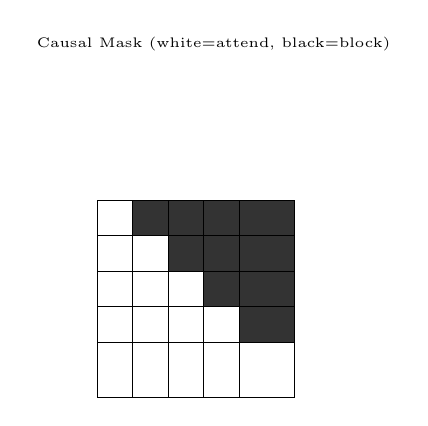
\begin{tikzpicture}[scale=0.45, every node/.style={font=\tiny}]
  \node at (2.5, 5.2) {Causal Mask (white=attend, black=block)};
  \foreach \i in {0,...,4} {
    \foreach \j in {0,...,4} {
      \pgfmathtruncatemacro{\val}{\j <= \i ? 1 : 0}
      \ifnum\val=1
        \node[draw, fill=white, minimum size=0.7cm] at (\j, -\i) {};
      \else
        \node[draw, fill=black!80, text=white, minimum size=0.7cm] at (\j, -\i) {};
      \fi
    }
  }
\end{tikzpicture}

The masked attention computation is:

\[
  \text{Attention}(Q, K, V) = \text{softmax}\!\left(\frac{QK^\top}{\sqrt{d_k}} + \text{mask}\right)V
\]

\begin{pseudocode}[Causal (Masked) Self-Attention]
def causal_self_attention(Q: Tensor, K: Tensor, V: Tensor) -> Tensor:
    # Q: [batch, seq_len, d_k], K: [batch, seq_len, d_k], V: [batch, seq_len, d_v]
    d_k = Q.size(-1)
    seq_len = Q.size(-2)
    scores = Q @ K.transpose(-2, -1)  # [batch, seq_len, d_k] @ [batch, d_k, seq_len] -> [batch, seq_len, seq_len]
    scaled_scores = scores / math.sqrt(d_k)  # [batch, seq_len, seq_len]
    # Create causal mask: upper triangle is True (positions to block)
    mask = torch.triu(torch.ones(seq_len, seq_len, dtype=torch.bool), diagonal=1)  # [seq_len, seq_len]
    scaled_scores = scaled_scores.masked_fill(mask, float('-inf'))  # [batch, seq_len, seq_len]
    attn_weights = softmax(scaled_scores, dim=-1)  # [batch, seq_len, seq_len]
    output = attn_weights @ V  # [batch, seq_len, seq_len] @ [batch, seq_len, d_v] -> [batch, seq_len, d_v]
    return output
\end{pseudocode}

\begin{keyconcept}
  We use \texttt{masked\_fill} to directly set blocked positions to
  $-\infty$ in the score matrix. This matters because the alternative---multiplying
  a 0/1 mask into the scores---would produce NaN when 0 is multiplied by
  $-\infty$: $0 \times (-\infty) = \text{NaN}$. The \texttt{masked\_fill}
  operation sidesteps this by never computing $0 \times (-\infty)$; it simply
  replaces the blocked positions with $-\infty$ before softmax is applied.
  Some implementations add the mask as an additive bias ($+\text{mask}$)
  where the mask contains $0$ for allowed positions and $-\infty$ for blocked
  positions---this is equivalent to \texttt{masked\_fill}.
\end{keyconcept}

\section{Multi-Head Attention}

A single attention head computes one set of attention weights, which means it
can learn only one pattern of relationships. In practice, language has many
kinds of relationships: grammatical subject--verb agreement, coreference
resolution, semantic relatedness, positional proximity, and more. Multi-head
attention addresses this by running $h$ parallel attention computations (``heads''),
each with its own Q/K/V projections, then concatenating and projecting the
results.

Instead of one large attention computation with dimension $d_{\text{model}}$,
multi-head attention splits the embedding dimension into $h$ heads of dimension
$d_k = d_{\text{model}} / h$. Each head can attend to different aspects of the
input independently. The outputs are concatenated and passed through a final
linear projection $W_O$ that lets heads interact and mix information.

The projection matrices have the following shapes:
\begin{itemize}
  \item $W_Q, W_K \in \mathbb{R}^{d_{\text{model}} \times d_k}$ (or $\mathbb{R}^{d_{\text{model}} \times d_{\text{model}}}$ when combined for all heads)
  \item $W_V \in \mathbb{R}^{d_{\text{model}} \times d_v}$ (usually $d_v = d_k$)
  \item $W_O \in \mathbb{R}^{d_{\text{model}} \times d_{\text{model}}}$ (projects concatenated heads back to embed dim)
\end{itemize}

\begin{pseudocode}[Multi-Head Attention]
def multi_head_attention(X: Tensor, n_heads: int) -> Tensor:
    # X: [batch, seq_len, embed_dim]
    # W_Q, W_K, W_V: [embed_dim, embed_dim], W_O: [embed_dim, embed_dim]
    batch, seq_len, embed_dim = X.shape
    d_k = embed_dim // n_heads

    # Project inputs to Q, K, V
    Q = X @ W_Q  # [batch, seq_len, embed_dim]
    K = X @ W_K  # [batch, seq_len, embed_dim]
    V = X @ W_V  # [batch, seq_len, embed_dim]

    # Reshape to separate heads: [batch, seq_len, embed_dim] -> [batch, n_heads, seq_len, d_k]
    Q = Q.view(batch, seq_len, n_heads, d_k).transpose(1, 2)
    K = K.view(batch, seq_len, n_heads, d_k).transpose(1, 2)
    V = V.view(batch, seq_len, n_heads, d_k).transpose(1, 2)

    # Compute attention for each head (in parallel via batched operations)
    # attn_output: [batch, n_heads, seq_len, d_k]
    attn_output = scaled_dot_product_attention(Q, K, V)

    # Concatenate heads: [batch, n_heads, seq_len, d_k] -> [batch, seq_len, embed_dim]
    attn_output = attn_output.transpose(1, 2).contiguous().view(batch, seq_len, embed_dim)

    # Final output projection lets heads interact
    output = attn_output @ W_O  # [batch, seq_len, embed_dim]
    return output
\end{pseudocode}

\begin{keyconcept}
  The reshaping pattern is the key to understanding multi-head attention:
  \begin{itemize}
    \item \textbf{Split}: $[\text{batch}, \text{seq}, \text{embed}] \rightarrow
          [\text{batch}, h, \text{seq}, d_k]$
    \item \textbf{Attend}: each head computes scaled dot-product attention
          independently
    \item \textbf{Concat}: $[\text{batch}, h, \text{seq}, d_k] \rightarrow
          [\text{batch}, \text{seq}, \text{embed}]$
  \end{itemize}
  The output projection $W_O$ is essential---without it, heads cannot
  interact and mix information. Removing $W_O$ would mean the concatenated
  heads are simply stacked side-by-side with no cross-head communication.
\end{keyconcept}

Why not just use a single head with a larger dimension? The answer is
expressiveness. With $h$ heads, each of dimension $d_k = d_{\text{model}}/h$,
the model learns $h$ different attention patterns in parallel. Empirically,
multi-head attention significantly outperforms single-head attention at the
same total dimensionality.

\section{Attention as Soft Dictionary Lookup}

The Q/K/V formulation can be understood through the lens of a \emph{soft
dictionary}: a differentiable generalization of a hash table or database
lookup. The database analogy from Section~2 applies here too, but now we can
see how it plays out \emph{across layers} of a deep network.

In a standard dictionary, the lookup returns exactly one value (hard match).
Attention returns a distribution over values (soft match). This softness is
what makes attention differentiable: the gradients flow through all
value contributions proportionally to their attention weights.

\begin{keyconcept}
  \textbf{Layer depth matters}: early layers tend to capture local
  syntactic patterns (e.g., attending to adjacent words), while later
  layers capture broader semantic relationships (e.g., resolving pronoun
  references across long distances). This progression emerges naturally
  from training---the model learns that local patterns are easiest to model
  first and gradually builds up to longer-range dependencies.
\end{keyconcept}

\section{\texorpdfstring{$O(n^2)$}{O(n²)} Complexity and Modern Solutions}

The attention matrix is $n \times n$, where $n$ is the sequence length. This
gives:
\begin{itemize}
  \item \textbf{Time}: $O(n^2 d)$ for computing attention scores (every pair of
        positions, each with a $d$-dimensional dot product)
  \item \textbf{Space}: $O(n^2)$ for storing the attention matrix
\end{itemize}

For a 128K-token context, that is approximately 16 billion entries per attention
matrix, multiplied by the number of layers and heads. This quadratic scaling is
the primary bottleneck for long-context models.

To put this in perspective: a single attention layer with $n = 128{,}000$ tokens
requires $\sim\!128000^2 = 16.4$ billion floating-point values for the attention
matrix alone, consuming about 64~GB of memory (in float32). With multiple layers
and heads, long-context inference becomes prohibitively expensive without
optimization.

Modern solutions include:

\begin{center}
\begin{tabular}{ll}
\toprule
\textbf{Technique} & \textbf{Effect} \\
\midrule
KV Cache & Avoids recomputing past K/V during generation \\
Grouped Query Attention (GQA) & Reduces KV head count \\
Flash Attention & IO-aware algorithm, same $O(n^2)$ but faster \\
Sliding Window Attention & Limits attention to local context of width $w$, reducing to $O(nw)$ \\
Linear Attention & Approximates softmax for $O(n)$ time and space \\
\bottomrule
\end{tabular}
\end{center}

\begin{keyconcept}
  \textbf{KV Cache} is perhaps the most impactful practical optimization.
  During autoregressive generation, each new token must attend to all previous
  tokens. Without caching, this means recomputing the keys and values for all
  previous positions at every step. With caching, the keys and values for
  previous positions are stored and only the new position's K/V are computed.
  This reduces the per-step cost from $O(n^2)$ to $O(n)$ during generation
  (though training still requires the full $O(n^2)$ computation).

  \textbf{Grouped Query Attention (GQA)} reduces the memory bottleneck by
  sharing keys and values across multiple query heads. Instead of $h$ separate
  KV pairs, GQA uses $g < h$ groups, each sharing one KV pair. This reduces
  the KV cache size by a factor of $h/g$.

  \textbf{Flash Attention} is an IO-aware algorithm that avoids materializing
  the full $n \times n$ attention matrix in GPU global memory. It computes
  attention in tiles, keeping partial results in faster SRAM. The algorithmic
  complexity remains $O(n^2)$, but the wall-clock time is dramatically
  reduced because it avoids the bottleneck of writing and reading the massive
  attention matrix from slow memory.

  \textbf{Sliding Window Attention} restricts each position to attend only to
  the $w$ most recent positions, reducing both time and space to $O(nw)$. This
  trades global context for efficiency; some models combine it with a few
  global attention tokens to retain long-range information.

  \textbf{Linear Attention} replaces the softmax with a kernel-based
  approximation $\text{sim}(q, k) = \phi(q)^\top \phi(k)$ that allows the
  computation to be reordered as $\phi(V)(\phi(K)^\top \phi(Q))$, eliminating
  the $n \times n$ matrix entirely. The result is $O(n)$ time and space, but
  the approximation quality is still an open research question.
\end{keyconcept}

The attention mechanism you have built in this chapter---scaled dot-product
attention with causal masking, organized into multiple heads---is the core
computational primitive of the transformer. The next chapter assembles this
primitive into a complete architecture: the GPT-2 model, wrapping attention
in residual connections, layer normalization, and feed-forward layers to form
the full transformer block.

\section*{Review Questions}

\begin{reviewquestion}[1]
  Why does scaled dot-product attention divide by $\sqrt{d_k}$ rather
  than $d_k$? What would happen with $\sqrt{d_k}$ omitted for a model
  with $d_k = 64$?
\end{reviewquestion}

\begin{reviewquestion}[2]
  Explain why the output projection $W_O$ in multi-head attention is
  necessary. What would happen if you removed it and just concatenated
  the heads?
\end{reviewquestion}

\begin{reviewquestion}[3]
  Consider a causal language model processing a 128K-token context.
  Assuming 12 layers and 12 heads per layer, how many $n \times n$
  attention matrices are computed during a single forward pass?
\end{reviewquestion}

\begin{reviewquestion}[4]
  Explain the difference between simplified self-attention and scaled
  dot-product attention. What do the learnable Q/K/V projections provide
  that raw embeddings cannot?
\end{reviewquestion}

\begin{reviewquestion}[5]
  In the causal mask, position $i$ is allowed to attend to position $j$
  when $j \leq i$. Why is the condition $j \leq i$ rather than $j < i$?
  What would happen if a position could not attend to itself?
\end{reviewquestion}

\begin{reviewquestion}[6]
  Using the database analogy, explain what the query, key, and value
  represent. Why is the result of attention a ``soft'' lookup rather
  than a ``hard'' lookup?
\end{reviewquestion}

\begin{reviewquestion}[7]
  Suppose you have a 6-token sequence and multi-head attention with
  3 heads and $d_{\text{model}} = 48$. What is the dimension of each
  head's Q, K, and V? What is the shape of the attention score matrix
  for a single head?
\end{reviewquestion}

\begin{reviewquestion}[8]
  Why does \texttt{masked\_fill} with $-\infty$ produce the correct
  causal mask, while multiplying by 0 could cause numerical issues?
  Explain with a concrete edge case.
\end{reviewquestion}

\begin{reviewquestion}[9]
  How does attention address the two main limitations of RNNs
  (sequential processing bottleneck and difficulty with long-range
  dependencies)?
\end{reviewquestion}

\begin{reviewquestion}[10]
  In multi-head attention, each head operates on dimension $d_k =
  d_{\text{model}} / h$. If you doubled the number of heads while
  keeping $d_{\text{model}}$ fixed, how would this affect the total
  number of parameters and the per-head computational cost?
\end{reviewquestion}

\begin{reviewquestion}[11]
  Explain how the KV cache works during autoregressive generation.
  Why does it reduce the per-step cost from $O(n^2)$ to $O(n)$?
\end{reviewquestion}

\begin{reviewquestion}[12]
  Grouped Query Attention (GQA) shares KV pairs across groups of query
  heads. Explain the tradeoff: what does GQA save, and what might it
  sacrifice?
\end{reviewquestion}

\begin{reviewquestion}[13]
  Why are three separate projection matrices ($W_Q$, $W_K$, $W_V$) used
  instead of a single shared projection? What capability would be lost
  if $W_K = W_V$?
\end{reviewquestion}

\begin{reviewquestion}[14]
  When implementing softmax from scratch, why must you subtract the
  maximum value before exponentiating? What would happen numerically
  with $d_k = 64$ and unscaled dot products if you skipped this step?
\end{reviewquestion}

\section*{Problems}

\begin{problem}[1]
  \textbf{Simplified Self-Attention from Scratch.}
  Implement simplified self-attention using only basic tensor operations
  (matrix multiplication and softmax---no \texttt{nn.Module} or learned
  parameters). Your function should take an input tensor of shape
  $[\text{batch}, \text{seq\_len}, \text{embed\_dim}]$ and return an output tensor of the
  same shape. Verify that each row of the attention weight matrix sums to 1.
\end{problem}

\begin{problem}[2]
  \textbf{Scaled Dot-Product Attention.}
  Implement scaled dot-product attention with learnable $W_Q$, $W_K$, $W_V$
  projections as \texttt{nn.Linear} modules. Write a function
  \texttt{scaled\_dot\_product\_attention(Q, K, V)} that computes
  $\text{softmax}(QK^\top / \sqrt{d_k})V$. Implement softmax from scratch
  (with max-subtraction for numerical stability) rather than using
  \texttt{torch.softmax}. Verify that removing the $\sqrt{d_k}$ scaling
  causes softmax to produce near-one-hot vectors for large $d_k$ (e.g.,
  $d_k = 256$).
\end{problem}

\begin{problem}[3]
  \textbf{Causal Masking.}
  Add causal masking to your scaled dot-product attention implementation.
  Create a boolean upper-triangular mask using \texttt{torch.triu} and
  apply it with \texttt{masked\_fill}. Feed a sequence of 8 tokens and
  verify that position $i$ in the output depends only on positions
  $0, 1, \ldots, i$ by checking that setting a future token to a
  different value does not change the output at position $i$.
\end{problem}

\begin{problem}[4]
  \textbf{Multi-Head Attention.}
  Implement multi-head attention by extending your single-head
  implementation. Use the reshape--transpose pattern to split the
  embedding dimension into $h$ heads, compute attention in parallel,
  and concatenate and project the result with $W_O$. Test with
  \texttt{embed\_dim = 48} and \texttt{n\_heads = 3}, verifying the
  output shape is $[\text{batch}, \text{seq\_len}, \text{embed\_dim}]$.
\end{problem}

\begin{problem}[5]
  \textbf{Attention Complexity Experiment.}
  Measure the wall-clock time of your multi-head attention implementation
  for sequence lengths $[128, 256, 512, 1024, 2048]$. Plot time vs.\
  sequence length. Does the empirical curve match the theoretical
  $O(n^2)$ prediction? How does the memory usage scale? Use
  \texttt{torch.cuda.max\_memory\_allocated()} if a GPU is available,
  or estimate memory from the size of the attention matrix.
\end{problem}